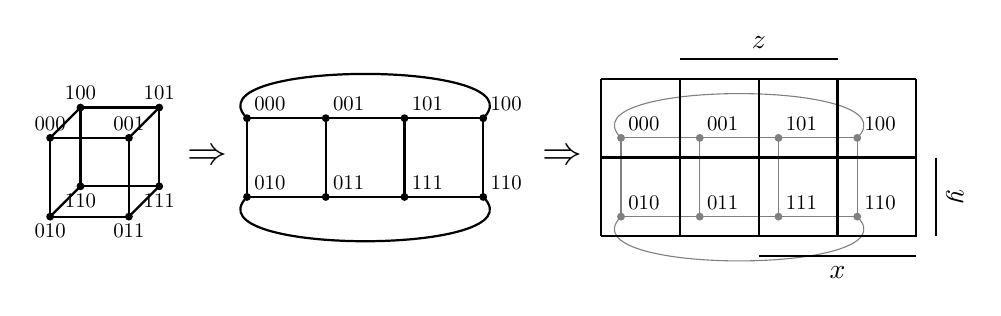
\begin{tikzpicture}
\begin{scope}[yshift=-0.25 cm]
\draw[thick] (0,0) node[scale=0.75,anchor=south]{000} -- (1,0) node[scale=0.75,anchor=south]{001} -- (1,-1) node[scale=0.75,anchor=north]{011} -- (0,-1) node[scale=0.75,anchor=north]{010} -- cycle;
\draw[thick] (0,0,-1) node[scale=0.75,anchor=south]{100} -- (1,0,-1) node[scale=0.75,anchor=south]{101} -- (1,-1,-1) node[scale=0.75,anchor=north]{111} -- (0,-1,-1) node[scale=0.75,anchor=north]{110} -- cycle;
\draw[thick] (0,0,0) -- (0,0,-1);
\draw[thick] (0,-1,0) -- (0,-1,-1);
\draw[thick] (1,0,0) -- (1,0,-1);
\draw[thick] (1,-1,0) -- (1,-1,-1);
\fill (0,0) circle(0.05 cm);
\fill (1,0) circle(0.05 cm);
\fill (1,-1) circle(0.05 cm);
\fill (0,-1) circle(0.05 cm);
\fill (0,0,-1) circle(0.05 cm);
\fill (1,0,-1) circle(0.05 cm);
\fill (1,-1,-1) circle(0.05 cm);
\fill (0,-1,-1) circle(0.05 cm);
\end{scope}
\draw (2,-0.5) node{\Large $\Rightarrow$};
\begin{scope}[xshift=2.5 cm]
\foreach\y in {0,1} {
  \foreach\z in {0,1} {
    \coordinate (N0\y\z) at (\z,-\y);
    \fill (N0\y\z) circle(0.05 cm) node[scale=0.75,anchor=south west]{0\y\z};
  }
}
\foreach\y in {0,1} {
  \foreach\z in {0,1} {
    \coordinate (N1\y\z) at (3-\z,-\y);
    \fill (N1\y\z) circle(0.05 cm) node[scale=0.75,anchor=south west]{1\y\z};
  }
}
\draw[thick] (N000) -- (N001) -- (N101) -- (N100) -- (N110) -- (N111) -- (N011) -- (N010) -- cycle;
\draw[thick] (N001) -- (N011);
\draw[thick] (N101) -- (N111);
\draw[thick] (N000) .. controls (-0.75,0.75) and (3.75,0.75) .. (N100);
\draw[thick] (N010) .. controls (-0.75,-1.75) and (3.75,-1.75) .. (N110);
\end{scope}
\draw (6.5,-0.5) node{\Large $\Rightarrow$};
\begin{scope}[xshift=7.25 cm, yshift=-0.25 cm]
\foreach\y in {0,1} {
  \foreach\z in {0,1} {
    \coordinate (N0\y\z) at (\z,-\y);
    \fill[gray] (N0\y\z) circle(0.05 cm) node[scale=0.75,black,anchor=south west]{0\y\z};
  }
}
\foreach\y in {0,1} {
  \foreach\z in {0,1} {
    \coordinate (N1\y\z) at (3-\z,-\y);
    \fill[gray] (N1\y\z) circle(0.05 cm) node[scale=0.75,black,anchor=south west]{1\y\z};
  }
}
\draw[gray] (N000) -- (N001) -- (N101) -- (N100) -- (N110) -- (N111) -- (N011) -- (N010) -- cycle;
\draw[gray] (N001) -- (N011);
\draw[gray] (N101) -- (N111);
\draw[gray] (N000) .. controls (-0.75,0.75) and (3.75,0.75) .. (N100);
\draw[gray] (N010) .. controls (-0.75,-1.75) and (3.75,-1.75) .. (N110);
\foreach\x in {0,1,2,3} {
  \foreach\y in {0,1} {
    \draw[thick] (\x-0.25,-\y+0.75) -- ++(1,0);
    \draw[thick] (\x-0.25,-\y+0.75) -- ++(0,-1);
  }
}
\draw[thick] (-0.25,-1.25) -| ++(4,2);
\draw [thick] (1.75,-1.5) to node[midway,below]{$x$} (3.75,-1.5);
\draw [thick] (0.75,1) to node[midway,above]{$z$} (2.75,1);
\draw [thick] (4,-0.25) to node[midway,sloped,above]{$y$} (4,-1.25);
\end{scope}
\end{tikzpicture}